\chapter{Curva caracteristica de los diodos}

\subsection{Polarizacion en directa}

\begin{figure}[H]
    \centering
    \begin{tikzpicture}
        \begin{axis}[
            width=12cm,
            height=8cm,
            xlabel={$V$ [V]},
            ylabel={$I$ [mA]},
            grid=both,
            minor tick num=1,
            extra x ticks={0.7},
            extra x tick style={
              grid style={red, thick, dashed},
              tick style={red},
              tick label style={red}
             },
            scaled ticks=false,
            restrict x to domain=-1:4,
        ]
        \addplot[
            color=blue,
            mark=none,
            thick,
        ] table[
            col sep=tab,
            header=true,
            x=V1,
            y expr=\thisrow{I(D1)}*1000
        ] {tables/1N4007Directa.txt};
        \end{axis}
    \end{tikzpicture}
    \caption{Curva del diodo 1N4007 en directa, obtenida por simulación.}
    \label{fig:1N4007Directa}
\end{figure}

\begin{figure}[H]
    \centering
    \begin{tikzpicture}
        \begin{axis}[
            width=12cm,
            height=8cm,
            xlabel={$V$ [V]},
            ylabel={$I$ [mA]},
            grid=both,
            minor tick num=1,
            extra x ticks={0.3},
            extra x tick style={
              grid style={red, thick, dashed},
              tick style={red},
              tick label style={red}
             },
            scaled ticks=false,
            restrict x to domain=-1:4,
        ]
        \addplot[
            color=blue,
            mark=none,
            thick,
        ] table[
            col sep=tab,
            header=true,
            x=V1,
            y expr=\thisrow{I(D1)}*1000
        ] {tables/1N60Directa.txt};
        \end{axis}
    \end{tikzpicture}
    \caption{Curva del diodo 1N60 en directa, obtenida por simulación.}
    \label{fig:1N60Directa}
\end{figure}

\begin{figure}[H]
    \centering
    \begin{tikzpicture}
        \begin{axis}[
            width=12cm,
            height=8cm,
            xlabel={$V$ [V]},
            ylabel={$I$ [mA]},
            grid=both,
            minor tick num=1,
            extra x ticks={0.3, 0.7},
            extra x tick style={
              grid style={red, thick, dashed},
              tick style={red},
              tick label style={red}
             },
            scaled ticks=false,
            restrict x to domain=-1:4,
            legend pos=north west,
        ]
        \addplot[
            color=blue,
            mark=none,
            thick,
        ] table[
            col sep=tab,
            header=true,
            x=V1,
            y expr=\thisrow{I(D1)}*1000
        ] {tables/1N60Directa.txt};
        \addlegendentry{1N60}
        \addplot[
            color=green,
            mark=none,
            thick,
        ] table[
            col sep=tab,
            header=true,
            x=V1,
            y expr=\thisrow{I(D1)}*1000
        ] {tables/1N4007Directa.txt};
        \addlegendentry{1N4007}
        \end{axis}
    \end{tikzpicture}
    \caption{Comparación de las curvas de los diodos 1N4007 y 1N60}
    \label{fig:ComparacionDirecta}
\end{figure}

\subsection{Polarizacion en inversa}

\begin{figure}[H]
    \centering
    \begin{tikzpicture}
        \begin{axis}[
            width=12cm,
            height=8cm,
            xlabel={$V$ [kV]},
            ylabel={$I$ [mA]},
            grid=both,
            minor tick num=1,
            scaled ticks=false,
        ]
        \addplot[
            color=blue,
            mark=none,
            thick,
        ] table[
            col sep=tab,
            header=true,
            x expr=\thisrow{V1}/1000,
            y expr=\thisrow{I(D1)}*1000
        ] {tables/1N4007Inversa.txt};
        \end{axis}
    \end{tikzpicture}
    \caption{Curva del diodo 1N4007 en inversa, obtenida por simulación.}
    \label{fig:1N4007Inversa}
\end{figure}

\begin{figure}[H]
    \centering
    \begin{tikzpicture}
        \begin{axis}[
            width=12cm,
            height=8cm,
            xlabel={$V$ [V]},
            ylabel={$I$ [mA]},
            grid=both,
            minor tick num=1,
            scaled ticks=false,
            restrict x to domain=-50:10,
        ]
        \addplot[
            color=blue,
            mark=none,
            thick,
        ] table[
            col sep=tab,
            header=true,
            x = V1,
            y expr=\thisrow{I(D1)}*1000
        ] {tables/1N60Inversa.txt};
        \end{axis}
    \end{tikzpicture}
    \caption{Curva del diodo 1N60 en inversa, obtenida por simulación.}
    \label{fig:1N60Inversa}
\end{figure}

\section{Actividad de laboratorio}

\begin{figure}[H]
  \centering
  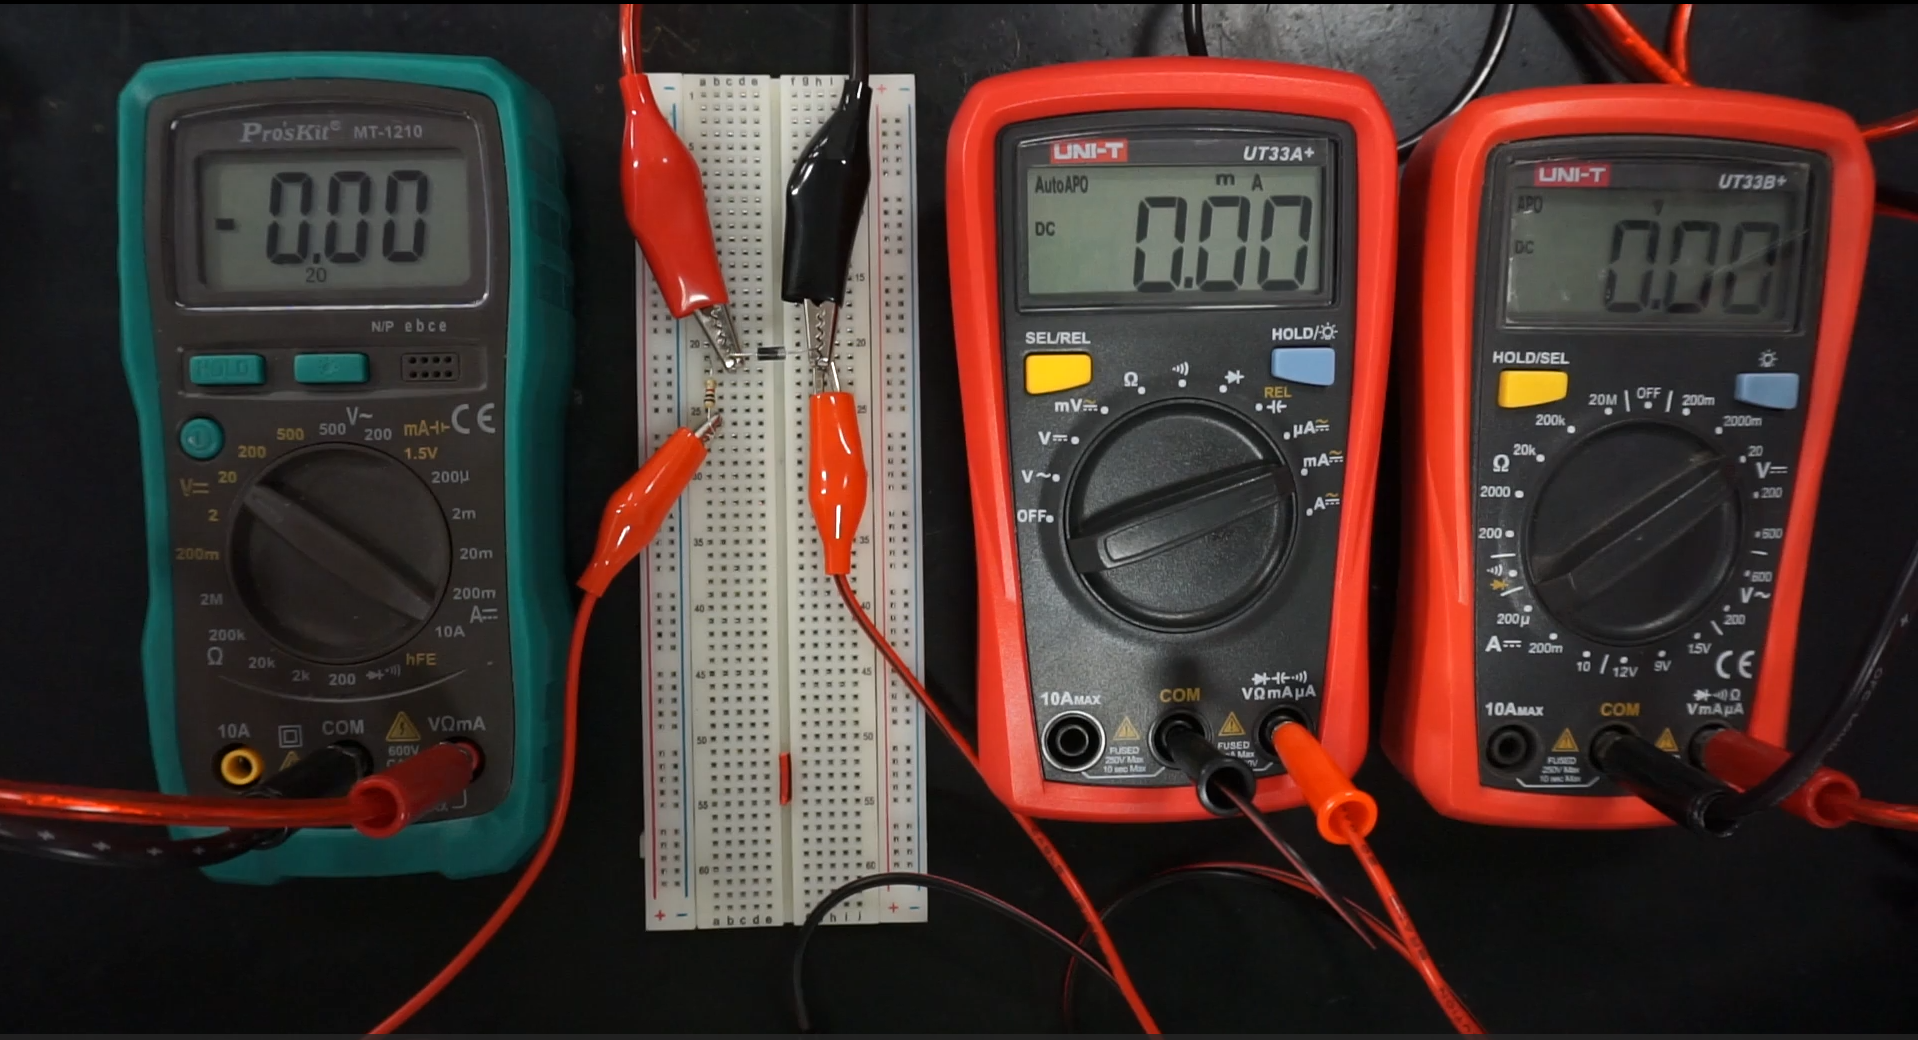
\includegraphics[width=0.7\textwidth]{images/circuitoN4007.png}
  \caption{Circuito del diodo 1N4007 en polarizacion directa}
\end{figure}

\begin{figure}[H]
  \centering
  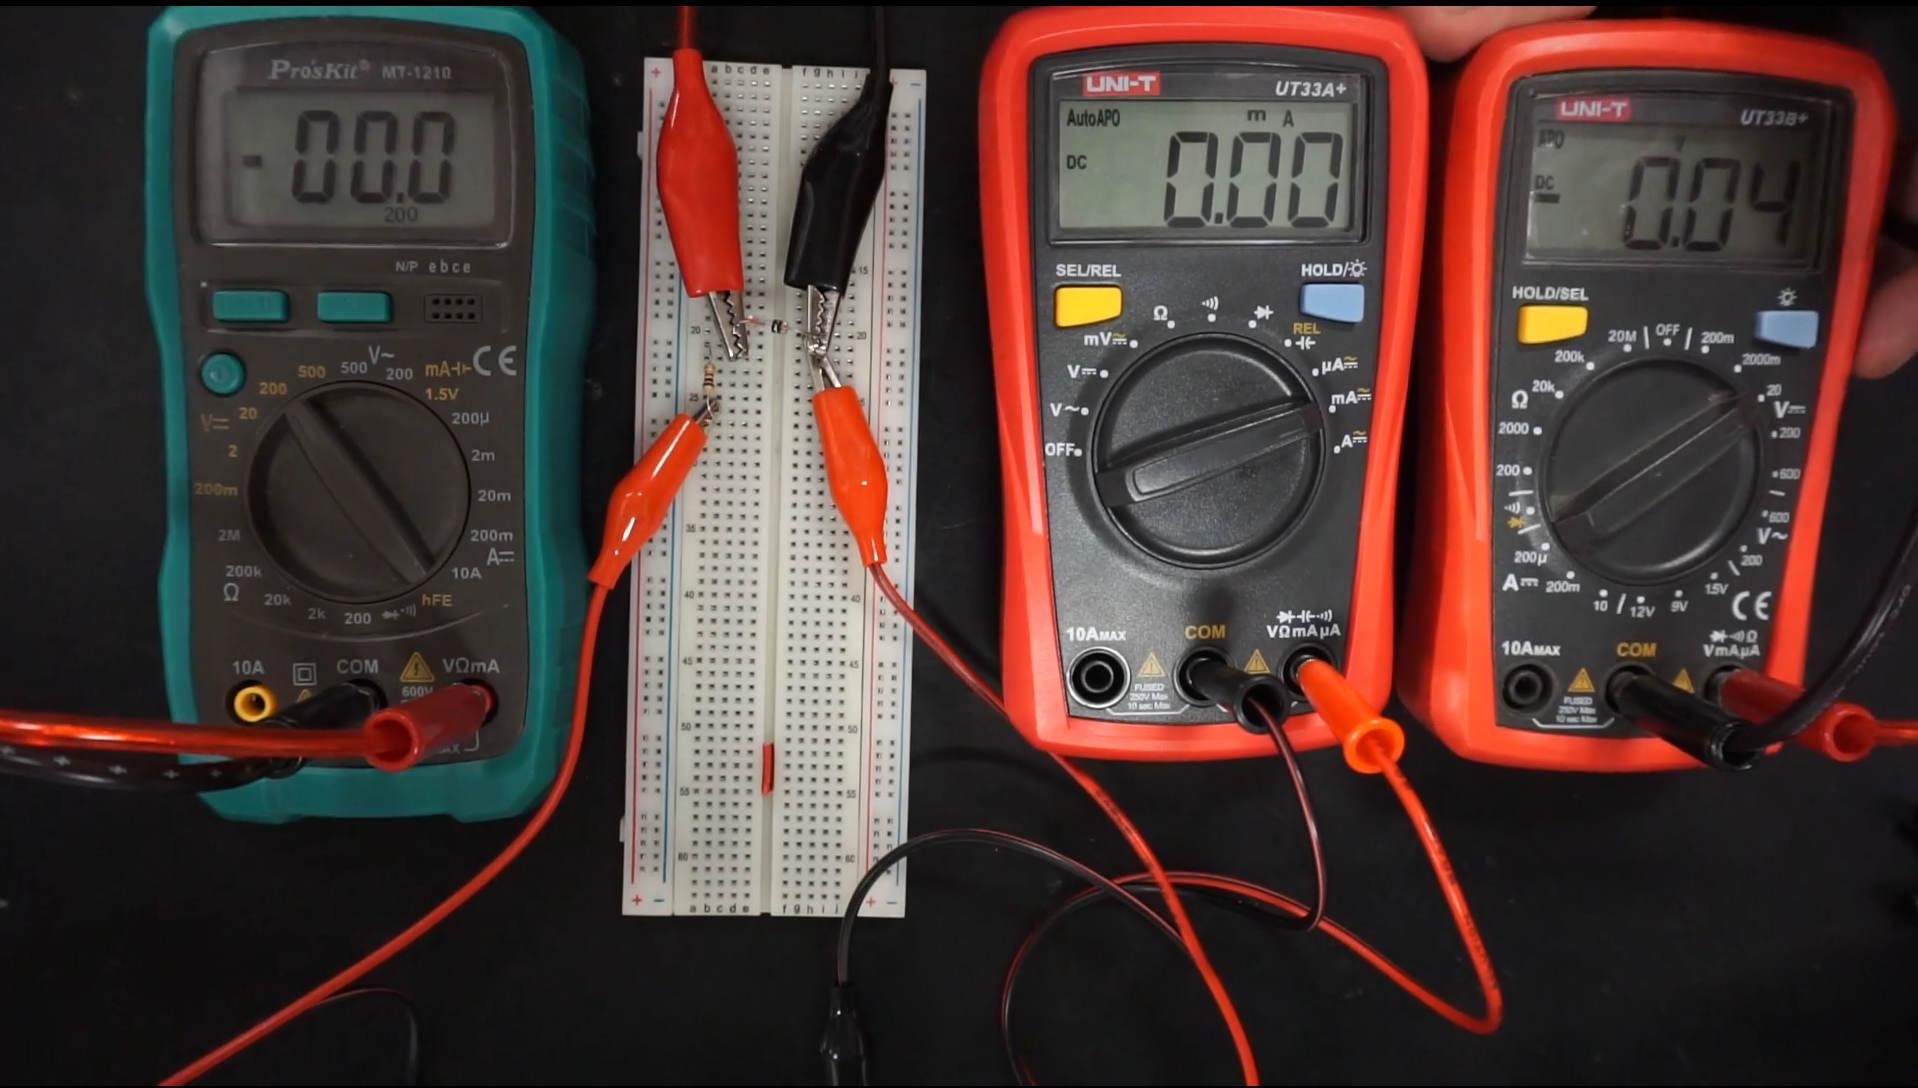
\includegraphics[width=0.7\textwidth]{images/circuitoN60.png}
  \caption{Circuito del diodo 1N60 en polarizacion directa}
\end{figure}

\begin{table}[H]
\centering
\begin{tabular}{|c|c|c|c|c|c|c|c|c|c|c|c|c|c|}
  \hline
  $V_1$ [V]   & 0 & 0.1 & 0.3 & 0.4 & 0.45 & 0.5 & 0.55 & 0.6 & 0.65 & 0.7 & 1 & 3 & 5 \\
  \hline
  $V_D$ [V]   & 0 & 0.19 & 0.24 & 0.31 &     &     &     &     &     &     &   &   &   \\
  \hline
  $I_D$ [mA]  & 0 & 0    & 0    &      & 0   &     &     &     &     &     &   &   &   \\
  \hline
\end{tabular}
\caption{Datos obtenidos en el diodo 1N4007}
\label{tab:diodo-datos}
\end{table}
